\documentclass[a4paper,11pt]{report}
\usepackage[T1]{fontenc}
\usepackage[utf8]{inputenc}
\usepackage[polish]{babel}
\usepackage{lmodern}
\usepackage{graphicx}

\title{Roznice w czasie realizacji algorytmów A star, DFS i BFS.}
\author{Arkadiusz Cyktor 200367}

\begin{document}
\maketitle

\begin{figure}
	1. Algorytm A star służy do odnajdywania najwydajniejszej ścieżki w grafie pomiędzy wierzchołkiem A i B. Do jego poprawnej realizacji potrzbna była funkcja heurystyczna, którą zaimplementowałem przez przypisanie wierzchołkom grafu współrzędnych kartezjańskich, co umożliwiło wyliczenie wspomnianej wcześniej funkcji, jako ich wzajemnej odległości w linii prostej. Taki sposób wyznaczania funkcji heurystycznej spełnia warunek, według którego nie powinna ona przeszacowywać odległości pomiędzy wierzchołkami. 
\end{figure}

\begin{figure}
  2. Poniższy wykres przedstawia zależność czasu potrzebnego na znalezienie zadanego wierzchołka grafu od ilości powtórzeń dla algorytmów \textbf{A star} (czerwony), \textbf{DFS} (zielony) i \textbf{BFS} (niebieski).
  \\\begin{center} 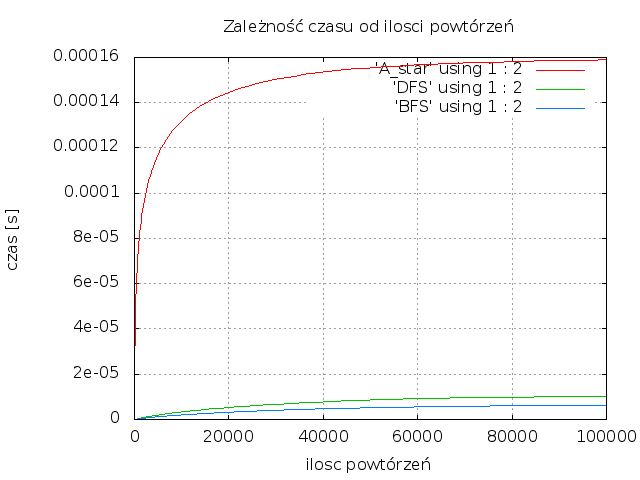
\includegraphics[scale=0.55]{./Razem.png}\end{center}
  Jak widać, wszystkie charakterystyki zmieniają się logarytmicznie, jednak najwięcej czesu na wykonanie obliczeń potrzebuje \textbf{A star}. Różnica pomiędzy przeszukiwaniem \textbf{w szerz}, a \textbf{w głąb} jest niewielka, widać jednak, że ten drugi okazał się wydajniejszy. Takie wyniki są spowodowane zasadniczą różnicą w działaniu wyżej wymienionch algorytmów - w \textbf{BFS} oraz \textbf{DFS} nie bierze się pod uwagę wag krawędzi łączących wierzchołki, co skutkuje wyszukaniem w dużo krótszym czasie, jednak wyznaczona ścieżka nie jest pierwszą znalezioną, a nie najlepszą z możliwych. \textbf{A star} wypada gorzej pod względem wydajności, ale jest dużo bardziej złożonym algorytmem, w którego wyniku otrzymujemy najbardziej optymalną ścieżkę, dlatego przed implementacją któregokolwiek z tych trzech algorytmów należy go dobrać odpowiednio do zastosowań. Jeśli zależy nam tylko na jak najkrótszym czasie odnalezienia drogi między A i B - wybierzemy \textbf{DFS} lub \textbf{BFS}, jeśli natomiast chcemy uzyskać najlepszy możliwy wynik, kosztem czasu obliczeń, nasz wybór padnie na \textbf{A star}.
\end{figure}

\begin{figure}
  \begin{center}
  Tabela z wynikami pomiarów:\\
  \begin{tabular}{|c|c|c|c|}
  \hline 
  Ilość powtórzeń & Czas - A star & Czas - DFS & Czas - BFS\\
  \hline
  10 & 0 & 0 & 0\\
  \hline
  100 & 0.0001 & 0 & 0\\
  \hline
  1000	&	0.00015 & 0 & 0\\
  \hline
  10000	&	0.000156 & 0.00001 & 0.000006\\
  \hline
  100000 &	0.000159 & 0.0000101 & 0.0000062\\
  \hline
\end{tabular}
\end{center}
\end{figure}
\end{document}